\subsection{Robustness}\label{subsec:robustnessoob}
We perform several robustness checks to assess the sensitivity of our results to various sample restrictions and different specifications. 

For our main specifications, we limited our sample to people who have been observed for a full 60 months. Since our data covers refugees who received protection up to August 2023, we can run our estimations with an extended sample, though the sample composition then changes with the outcome horizon.
Figure~\ref{fig:robustness_asylum2021} presents the results of our main findings without the restriction of being observed for 60 months. By including all refugees who received protection up to the start of 2021, our sample size increases to 45,666 individuals. The coefficients remain mostly unchanged, and the 95\% confidence intervals become slightly narrower for earlier months.

Second, we only consider refugees for whom we can determine in our data that they were in an initial reception facility at the beginning of their stay in Austria. For this group of 13,020 individuals, the assumption of exogenous placement is particularly credible. Figure~\ref{fig:rob_labor_mobility_initial_facility} shows the main results for this sample. Again, the overall patterns remain similar, with the effects of $IPBL$ on employment being somewhat smaller in magnitude.

In a related spirit, we exclude individuals who received protection within one month after first registering in Austria. This unusually quick process might still hint at individuals who came via family reunification.\footnote{In the main specification, we exclude individuals who received protection on the same day as they registered in Austria.} This tighter restriction excludes 2,036 observations, leaving a sample of 37,658 observations. However, results remain virtually unchanged (see Figure~\ref{fig:rob_labor_mobility_process_more1month}).

Third, we exclude individuals who received protection within four months of any of the welfare reforms. For these individuals, the $IPBL$ treatment is hard to interpret, as their benefit level changes immediately before/after receiving protection. As this concerns only 674 individuals, results hardly change from the main specification (see Figure~\ref{fig:rob_labor_mobility_noreform_4month}).

Fourth, we exclude individuals who moved between states in the month before receiving protection. This concerns 6,428 individuals. We suspect that these individuals already knew about the imminent granting of a protection status and moved preemptively. Figure~\ref{fig:rob_labor_mobility_state_approval_min1month} shows that excluding these observations leaves the results practically unchanged.

Fifth, we examine the robustness of inference to alternative clustering levels. Figure~\ref{fig:errors_all} shows 95\% confidence intervals at six choices: commuting zone, district, district $\times$ year, state, state $\times$ year-of-protection (our headline), and a wild-cluster bootstrap with Webb weights to address Austria's small number of states (nine). The two treatments vary at different aggregations---$IVUR$ at the district $\times$ month level, $IPBL$ at the state $\times$ protection-type $\times$ family-status $\times$ month level---and our headline state $\times$ year-of-protection cluster sits between these. It captures within-cohort residual correlation in placement, asylum-processing timing, and state-level policy environment. Under the wild-cluster bootstrap, which is the small-N-conservative choice with only nine states, confidence intervals widen and the band for the $IPBL$ effect on employment approaches zero at most horizons. We read this not as evidence that the $IPBL$ effect on employment is spurious but as a reminder that the statistical strength of that particular estimate is moderate; the $IPBL$ effect on mobility and the $IVUR$ effects throughout remain clearly distinguishable from zero across all clustering choices.

To ensure a particular nationality or state does not drive our results, we re-estimate the effects by systematically excluding either one nationality at a time (Figure~\ref{fig:leavenats}) or one state at a time (Figure~\ref{fig:leavestates}) in our main specification. In the leave-one-nationality-out analysis, the estimated effects remain largely unchanged, indicating robustness across different nationalities.
For the leave-one-state-out analysis, we modify our main specification by including an additional interaction of eligibility-for-family-benefits*state*type-of-protection. This adjustment is necessary since---otherwise---we would be using variation stemming from differences between refugee status (Convention vs. subsidiary protection) and eligibility for family benefits across states.  
Again, we see little change in our main results. If anything, the effects on mobility are larger when excluding Upper Austria (upper blue line) and are halved when excluding Vienna (lower blue line), likely due to the high concentration of refugees in this city.   

Finally, we use separate month and year-of-protection fixed effects instead of year-month fixed effects. This modification does not alter the results meaningfully (see Figure~\ref{fig:rob_labor_mobility_year_month_fe}).

Overall, we conclude that our results are robust to various changes in the sample and specification.

% \begin{figure}
%     \caption{Descriptive outcomes by moving behavior}
%     \label{fig:descriptive_outcomes_mover_group}
%     \begin{center}
%     \vspace{-0.5 cm}
%     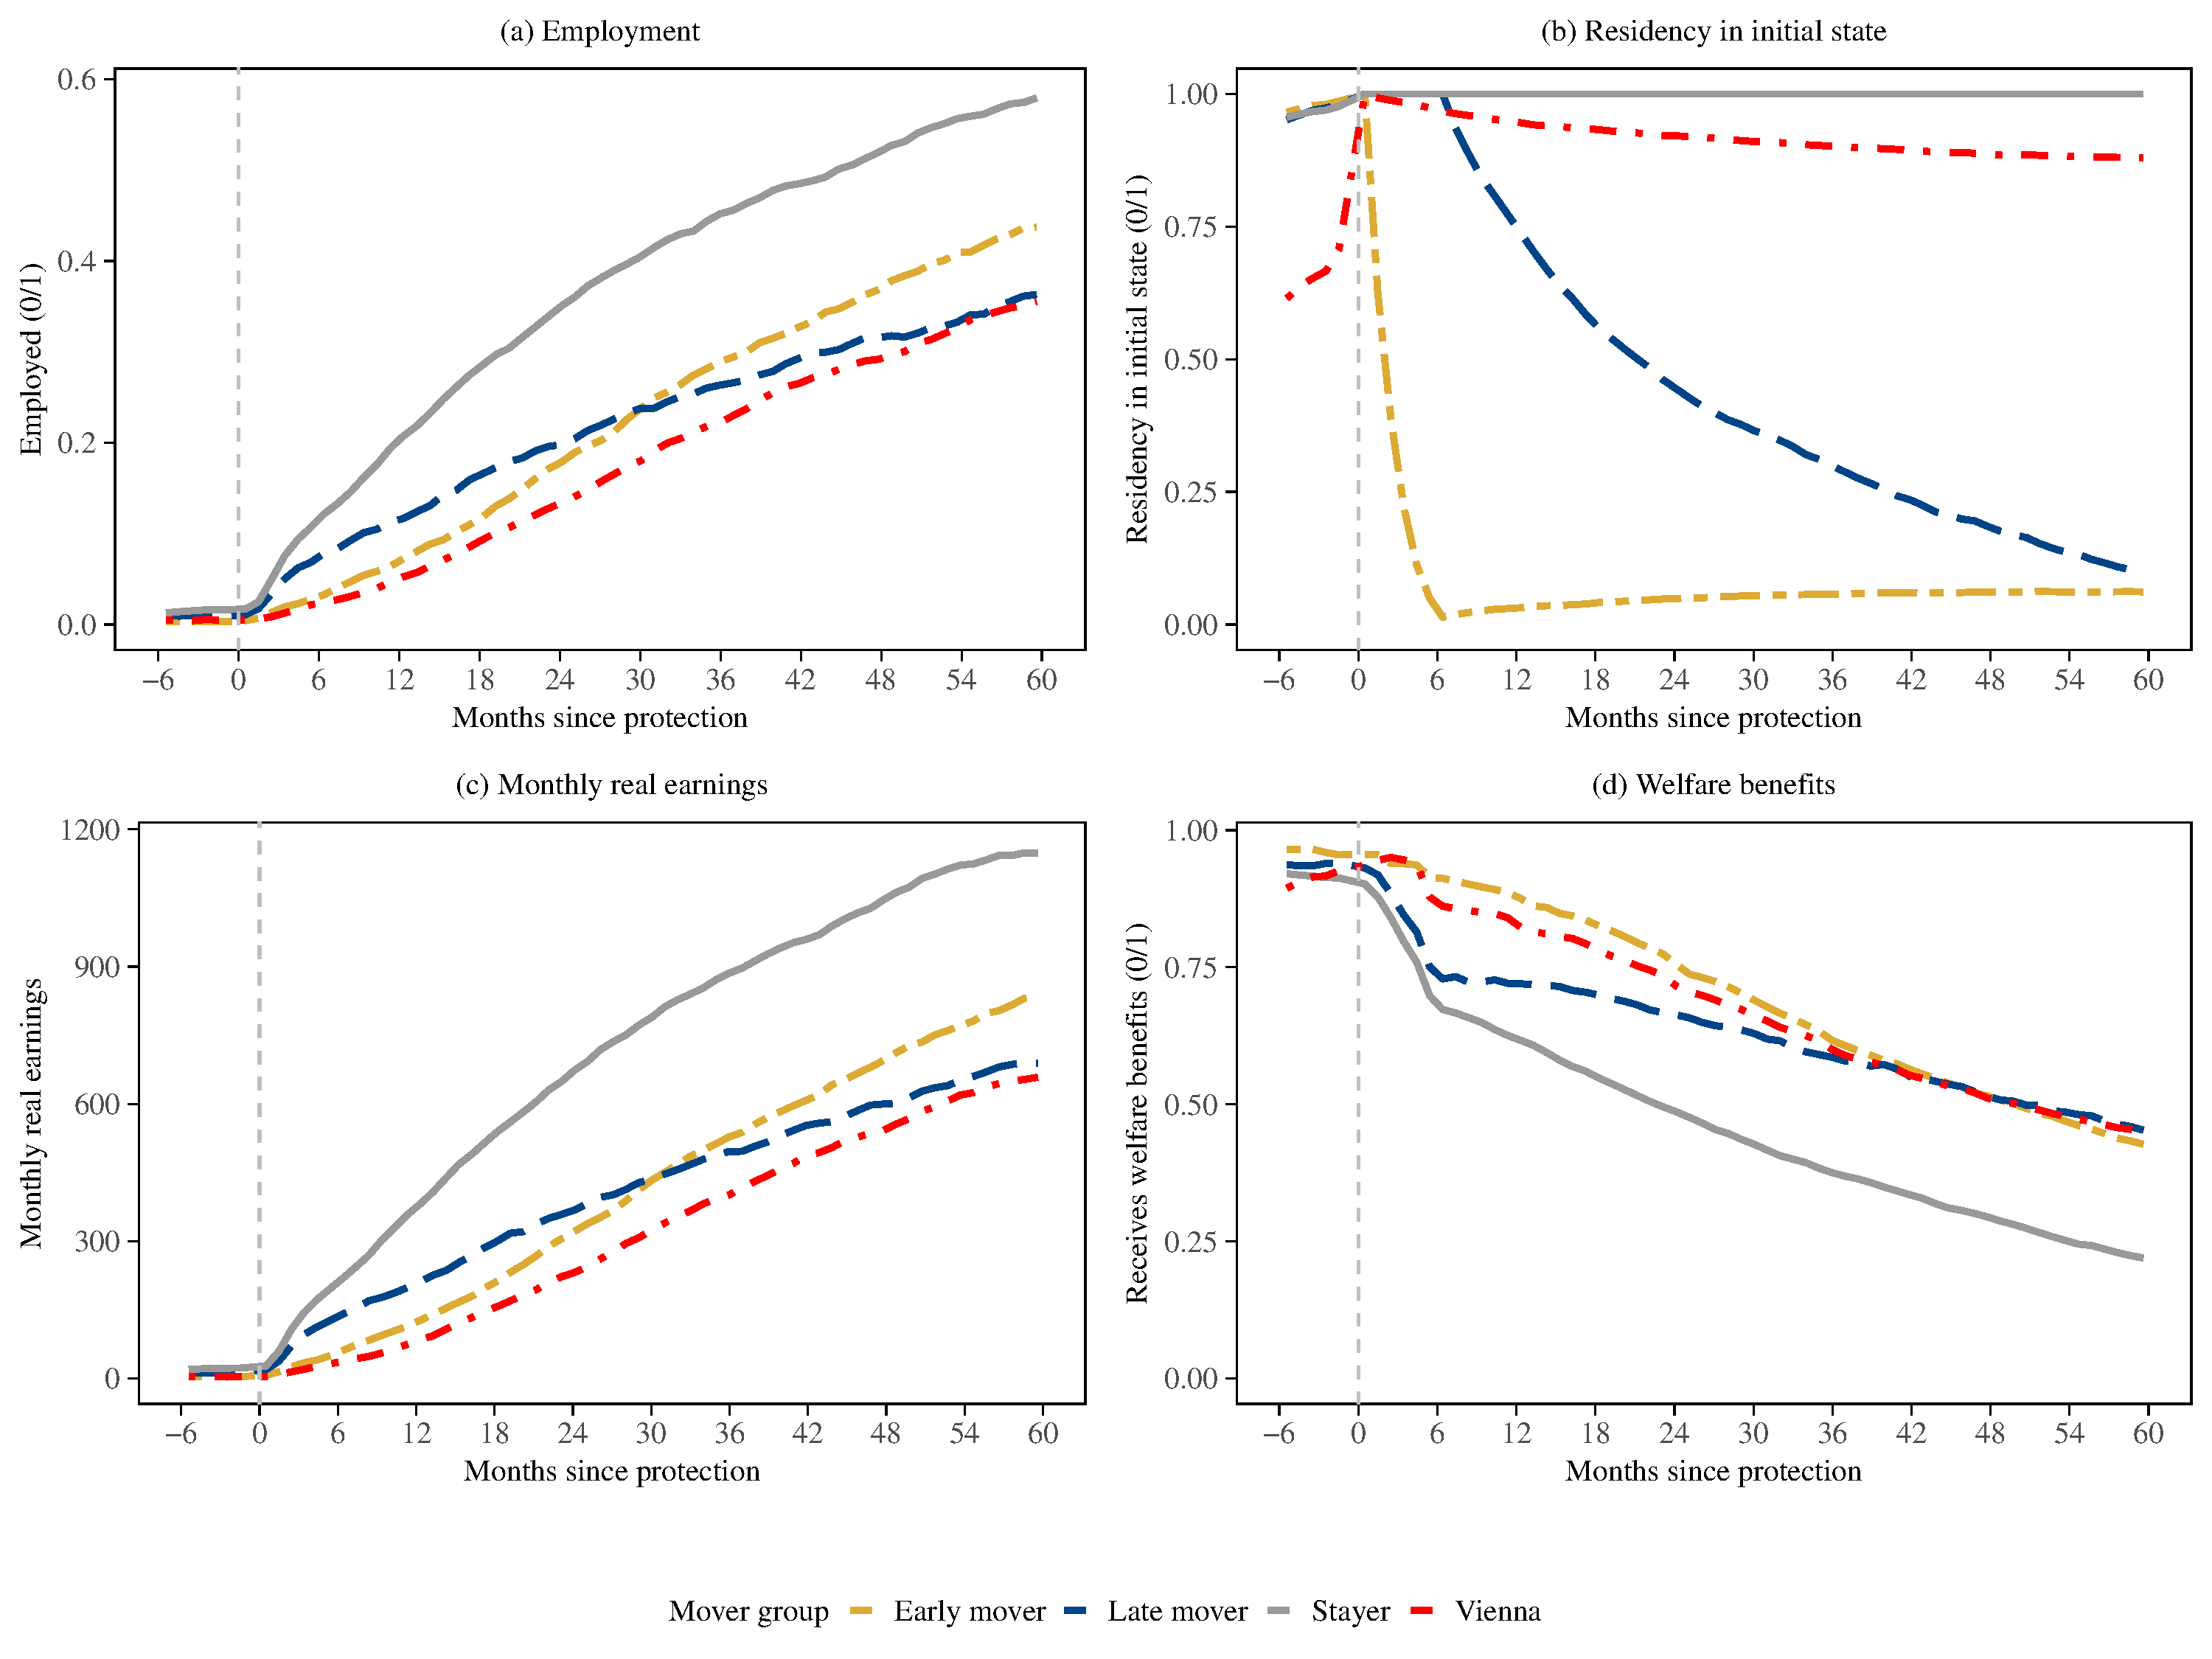
\includegraphics[scale=0.31]{figures/rob/fig_descriptive_outcomes_mover_group.pdf}
%     \end{center}
%     \fignote{Notes: The x-axis shows the months since protection was received. The y-axis displays descriptive outcomes for the groups categorized by their moving behavior.}
% \end{figure}

% \begin{figure}
%     \caption{Descriptive outcomes by moving behavior excluding people with relocation one month prior asylum granting}
%     \label{fig:mover_group_no_early}
%     \begin{center}
%     \vspace{-0.5 cm}
%     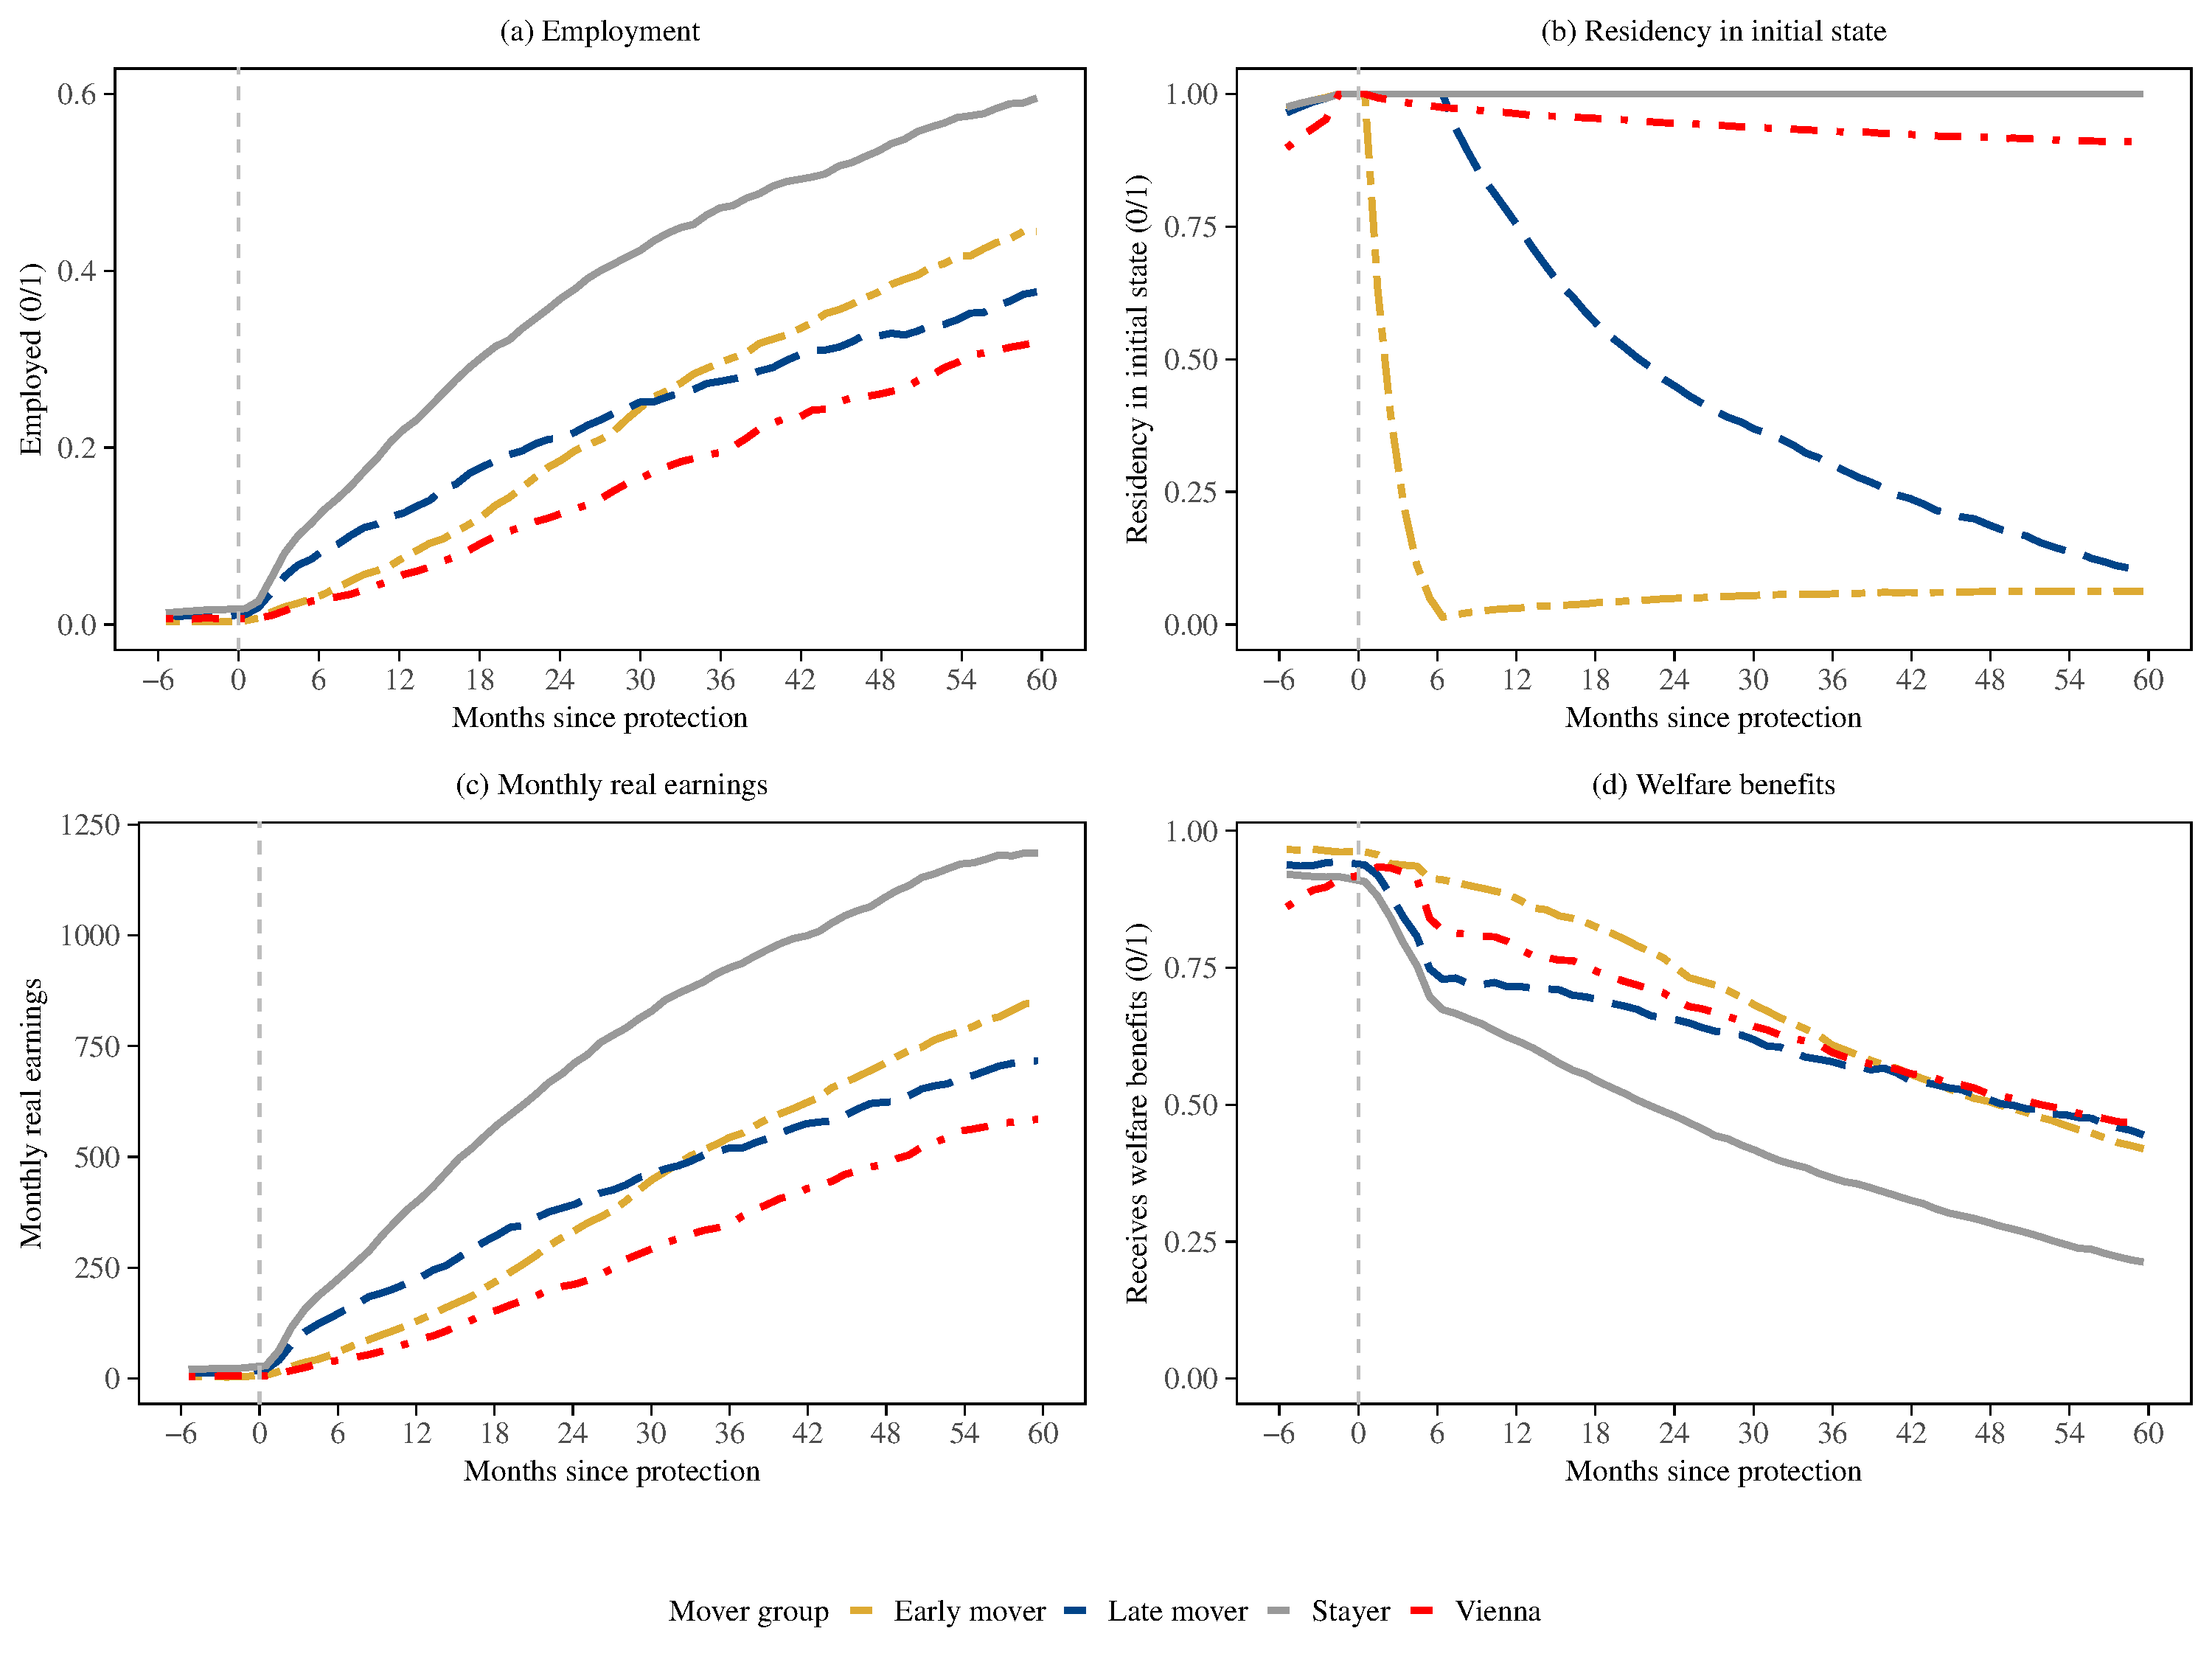
\includegraphics[scale=0.31]{figures/rob/fig_descriptive_outcomes_mover_group_no_early_movers.pdf}
%     \end{center}
%     \fignote{Notes: The x-axis shows the months since protection was received. The y-axis displays descriptive outcomes for the groups categorized by their moving behavior.}
% \end{figure}




% \begin{figure}
%     \caption{Effect of the $IVUR$ and $IPBL$ on employment and location choice with initial residency shifted to one month before receiving asylum}
%     \label{fig:rob_labor_mobility_initial_state_shift1}
%     \begin{center}
%     \vspace{-0.5 cm}
%     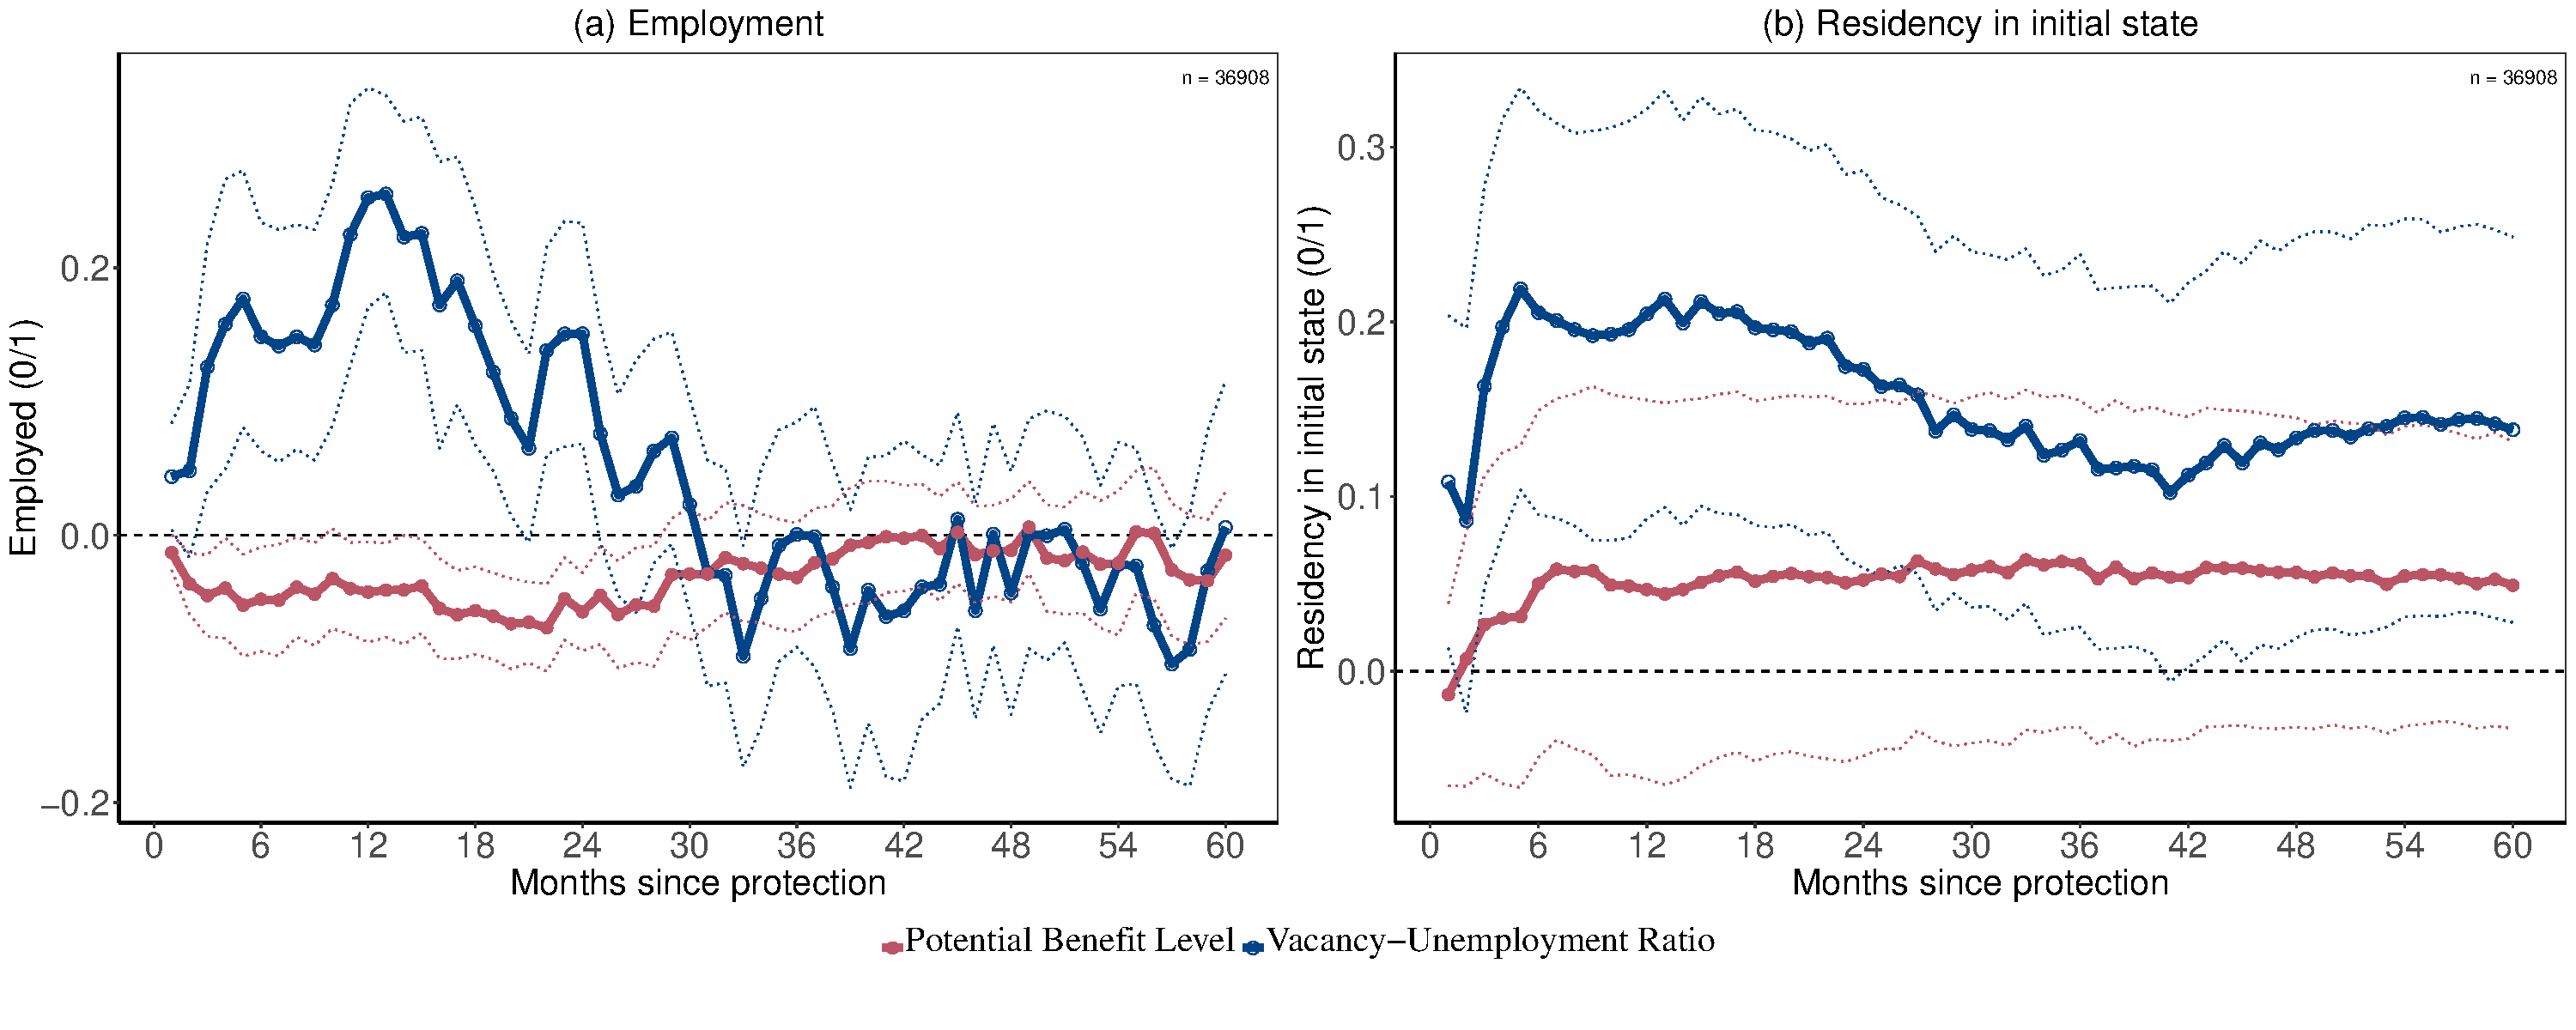
\includegraphics[scale=0.31]{figures/rob/fig_rob_labor_mobility_initial_state_shift1.pdf}
%     \end{center}
%     \fignote{Notes: The x-axis shows the months since protection was received. The y-axis displays the effect of a one-unit increase in either i) the vacancy-to-unemployment ratio or ii) the potential benefit level, measured in €1,000 (real 2015 values), on employment (left) and mobility (right). All regressions include a full set of arrival-group, year-month, and district-of-protection fixed effects. Additional control variables include age and age squared at immigration, gender, type of protection, family status at protection date, and country of origin. Standard errors are clustered at the district-year-of-protection level.}
% \end{figure}


% \begin{figure}
%     \caption{Effect of the $IVUR$  for the most desired professions and $IPBL$ on employment and location choice}
%     \label{fig:rob_labor_mobility_most_desired}
%     \begin{center}
%     \vspace{-0.5 cm}
%     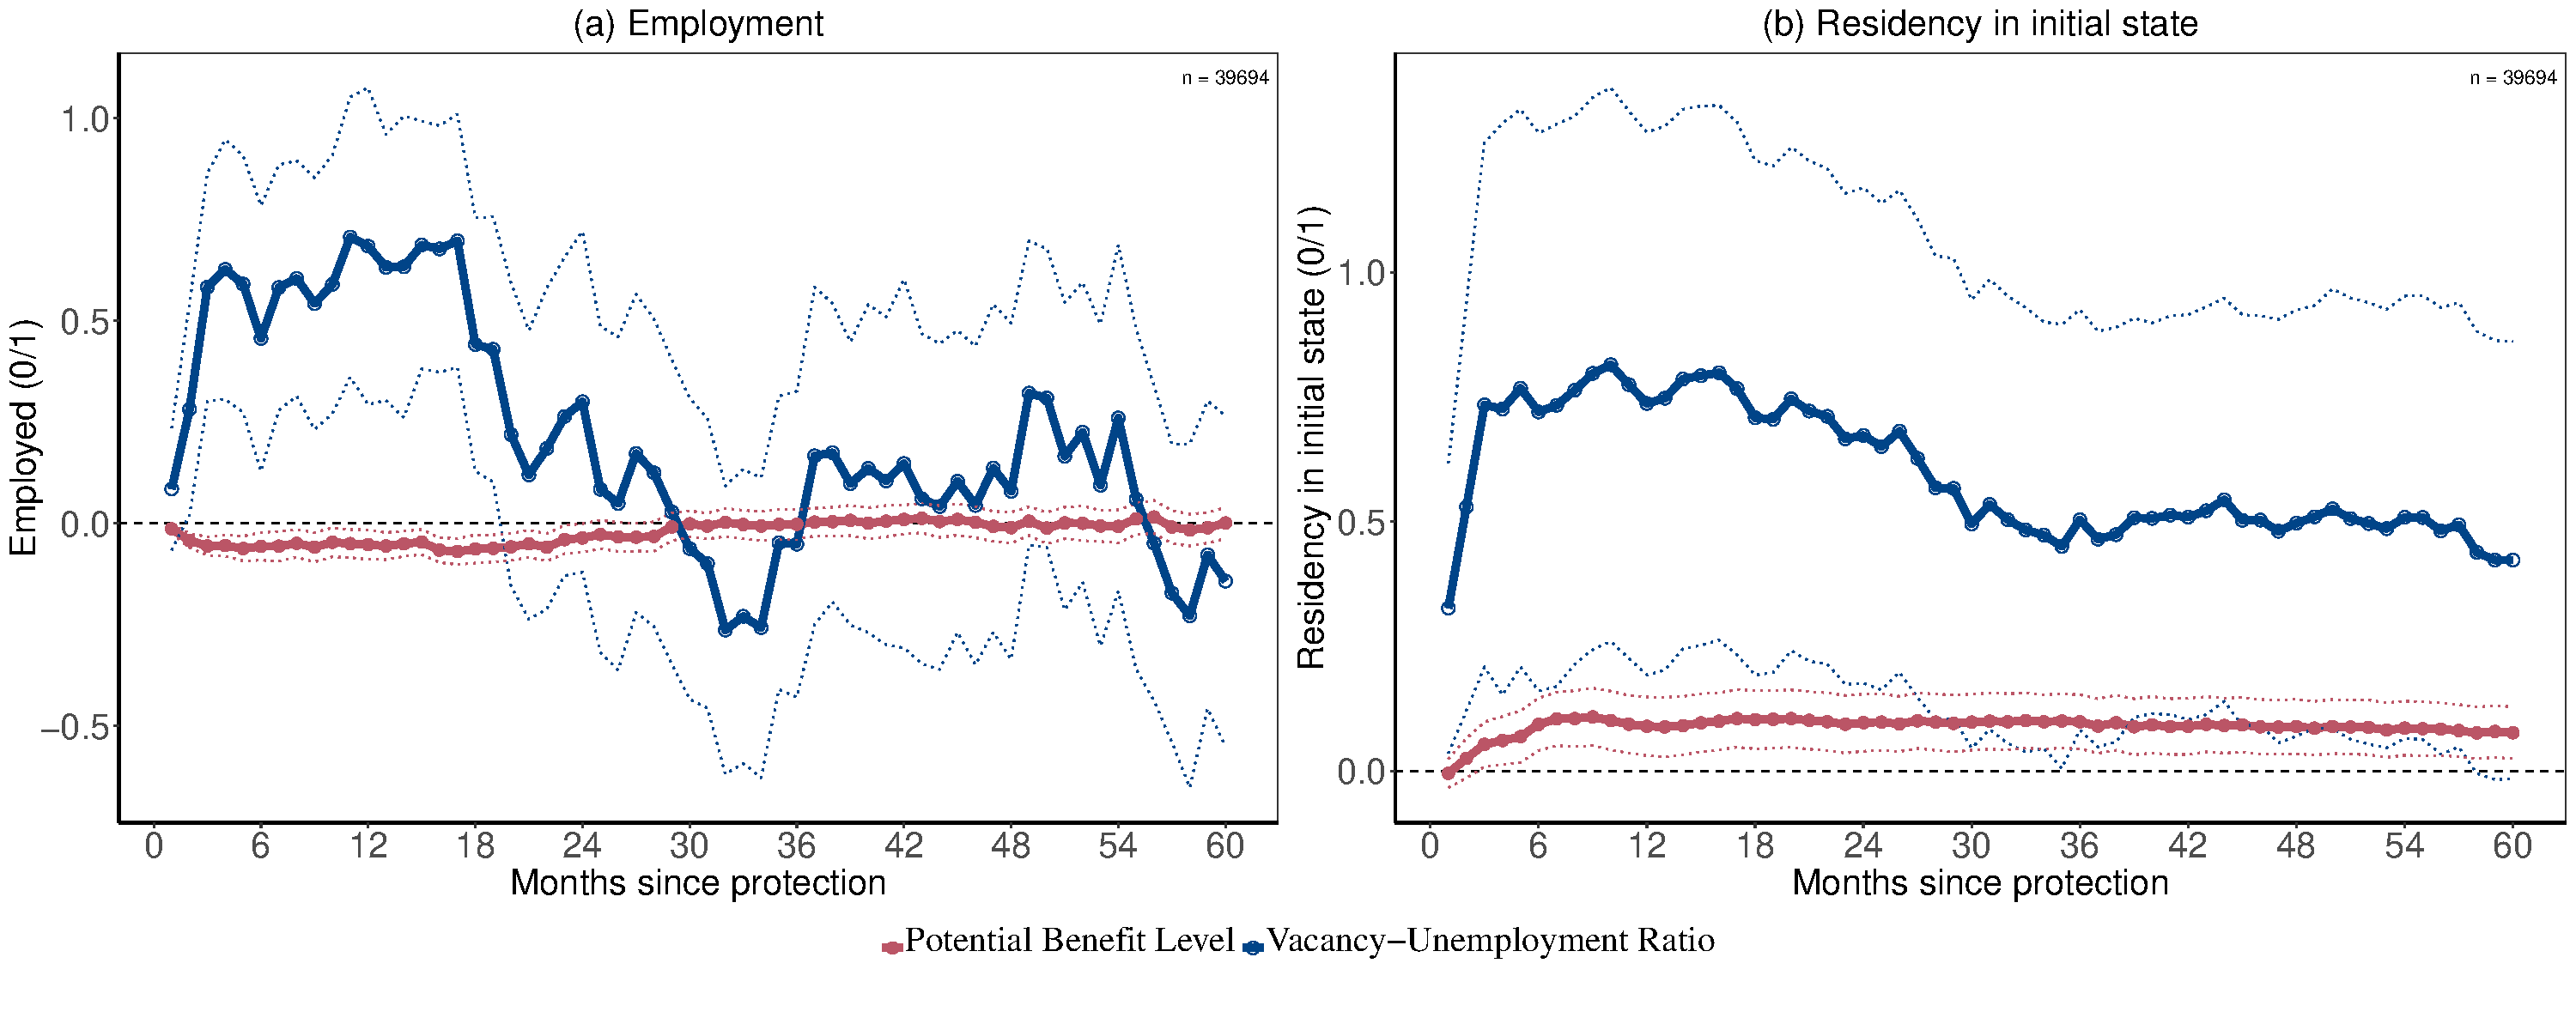
\includegraphics[scale=0.31]{figures/rob/fig_rob_labor_mobility_most_desired.pdf}
%     \end{center}
%     \fignote{Notes: The x-axis shows the months since protection was received. The y-axis displays the effect of a one-unit increase in either i) the occupation-specific vacancy-to-unemployment ratio or ii) the potential benefit level, measured in €1,000 (real 2015 values), on employment (left) and mobility (right). All regressions include a full set of arrival-group, year-month, and district-of-protection fixed effects. Additional control variables include age and age squared at immigration, gender, type of protection, family status at protection date, and country of origin. Standard errors are clustered at the district-year-of-protection level.}
% \end{figure}



% \begin{figure}
%     \caption{Effect of the $IVUR$ for seasonal professions and $IPBL$ on employment and location choice}
%     \label{fig:rob_labor_mobility_seasonal}
%     \begin{center}
%     \vspace{-0.5 cm}
%     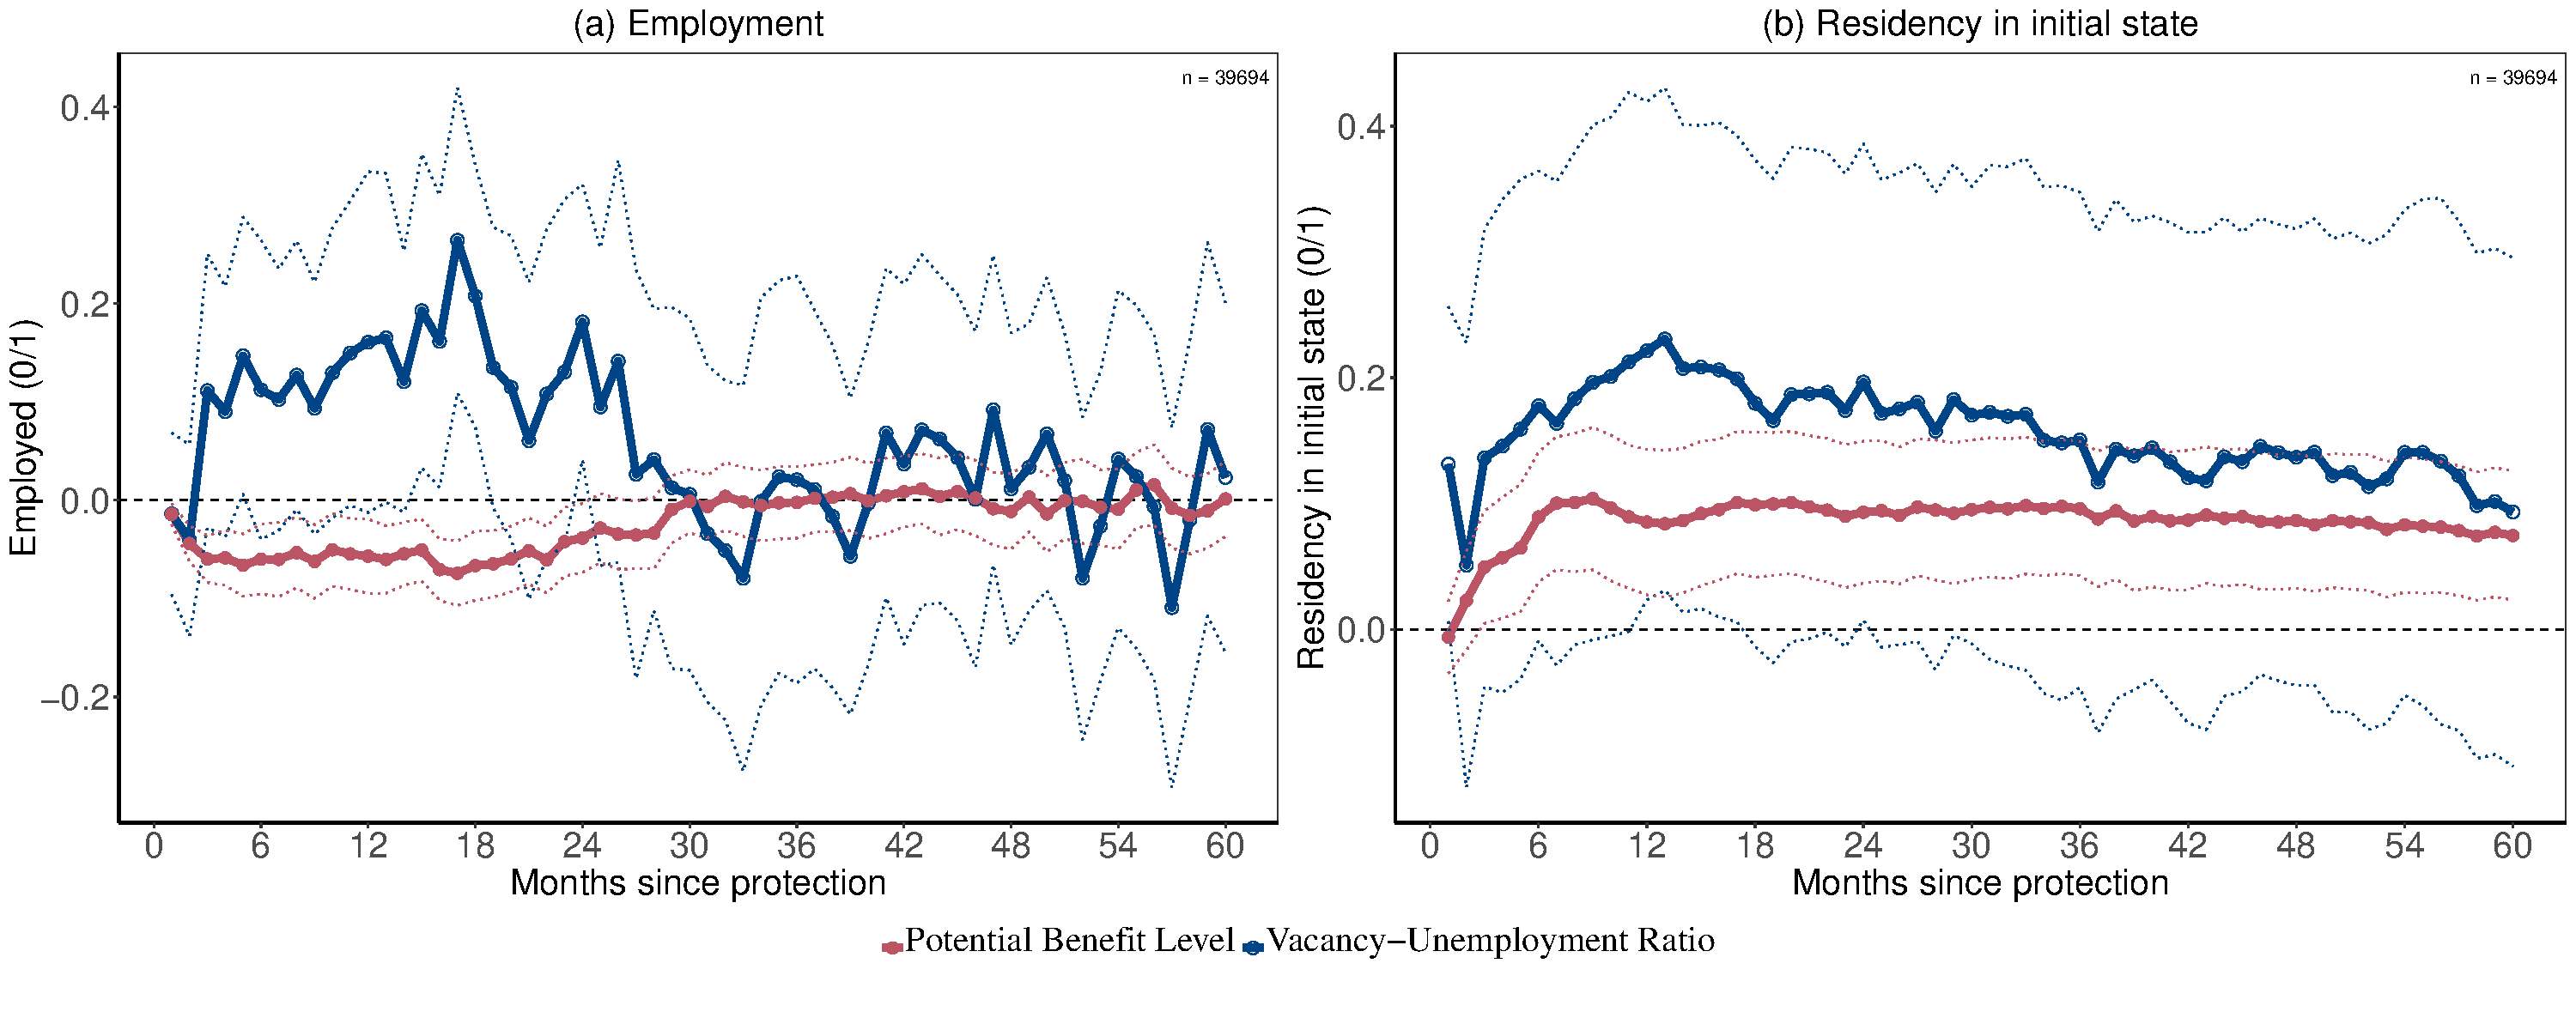
\includegraphics[scale=0.31]{figures/rob/fig_rob_labor_mobility_seasonal.pdf}
%     \end{center}
%     \fignote{Notes: The x-axis shows the months since protection was received. The y-axis displays the effect of a one-unit increase in either i) the occupation-specific vacancy-to-unemployment ratio or ii) the potential benefit level, measured in €1,000 (real 2015 values), on employment (left) and mobility (right). All regressions include a full set of arrival-group, year-month, and district-of-protection fixed effects. Additional control variables include age and age squared at immigration, gender, type of protection, family status at protection date, and country of origin. Standard errors are clustered at the district-year-of-protection level.}
% \end{figure}


% \begin{figure}
%     \caption{Pretrends: Effect of the $IVUR$ and $IPBL$ on employment and location choice}
%     \label{fig:rob_labor_mobility_pre_trends}
%     \begin{center}
%     \vspace{-0.5 cm}
%     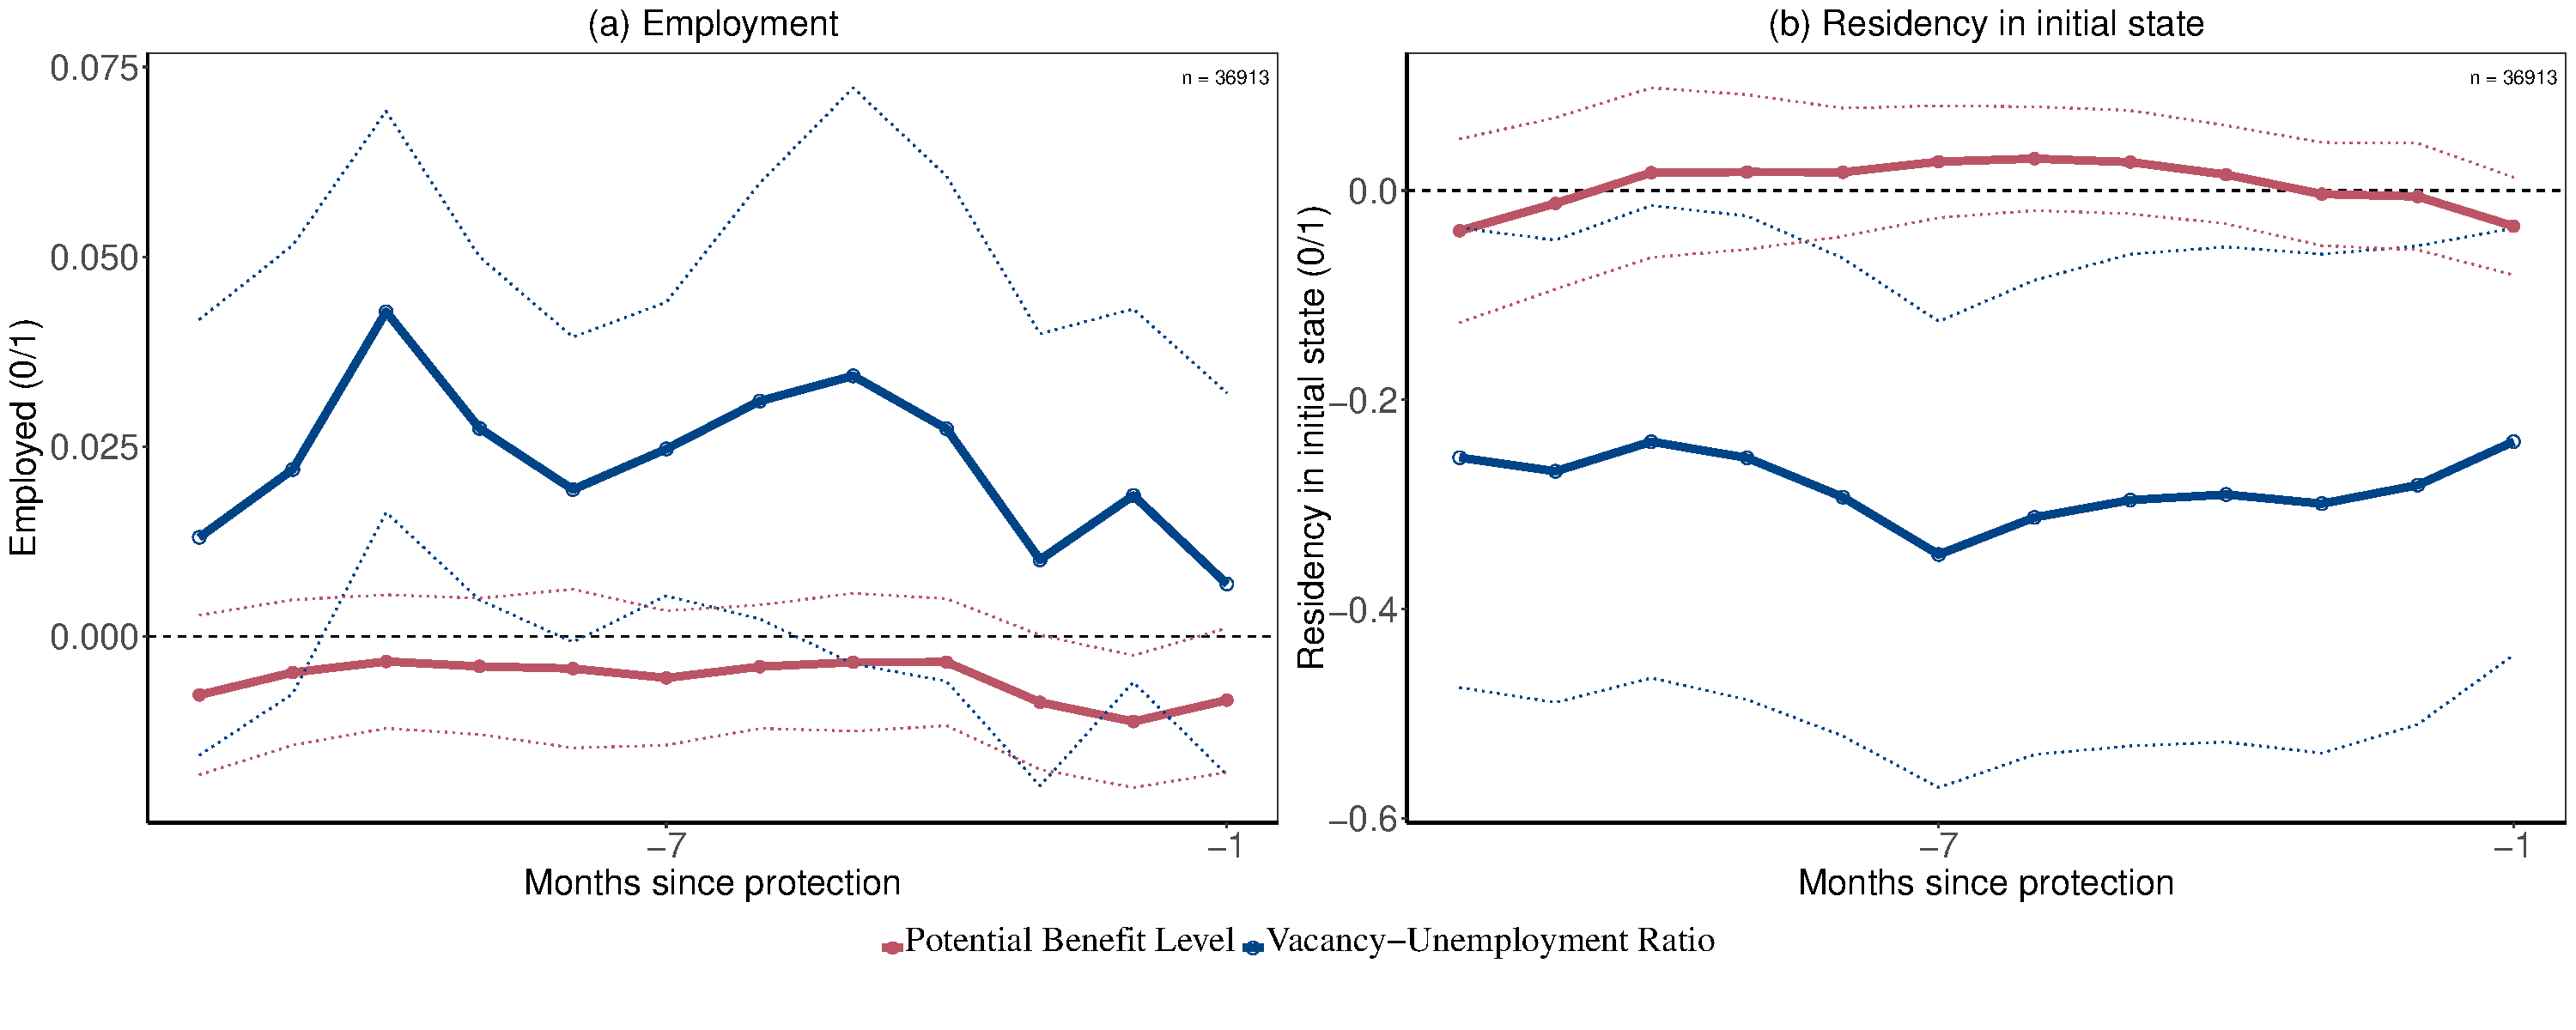
\includegraphics[scale=0.31]{figures/rob/fig_rob_labor_mobility_pre_trends.pdf}
%     \end{center}
%     \fignote{Notes: The x-axis shows the months since protection was received. The y-axis displays the effect of a one-unit increase in either i) the vacancy-to-unemployment ratio or ii) the potential benefit level, measured in €1,000 (real 2015 values), on employment (left) and mobility (right). All regressions include a full set of arrival-group, year-month, and district-of-protection fixed effects. Additional control variables include age and age squared at immigration, gender, type of protection, family status at protection date, and country of origin. Standard errors are clustered at the district-year-of-protection level.}
% \end{figure}

% \begin{figure}
%     \caption{Pretrends without early movers: Effect of the $IVUR$ and $IPBL$ on employment and location choice}
%     \label{fig:rob_labor_mobility_pre_trends_without_early_mover}
%     \begin{center}
%     \vspace{-0.5 cm}
%     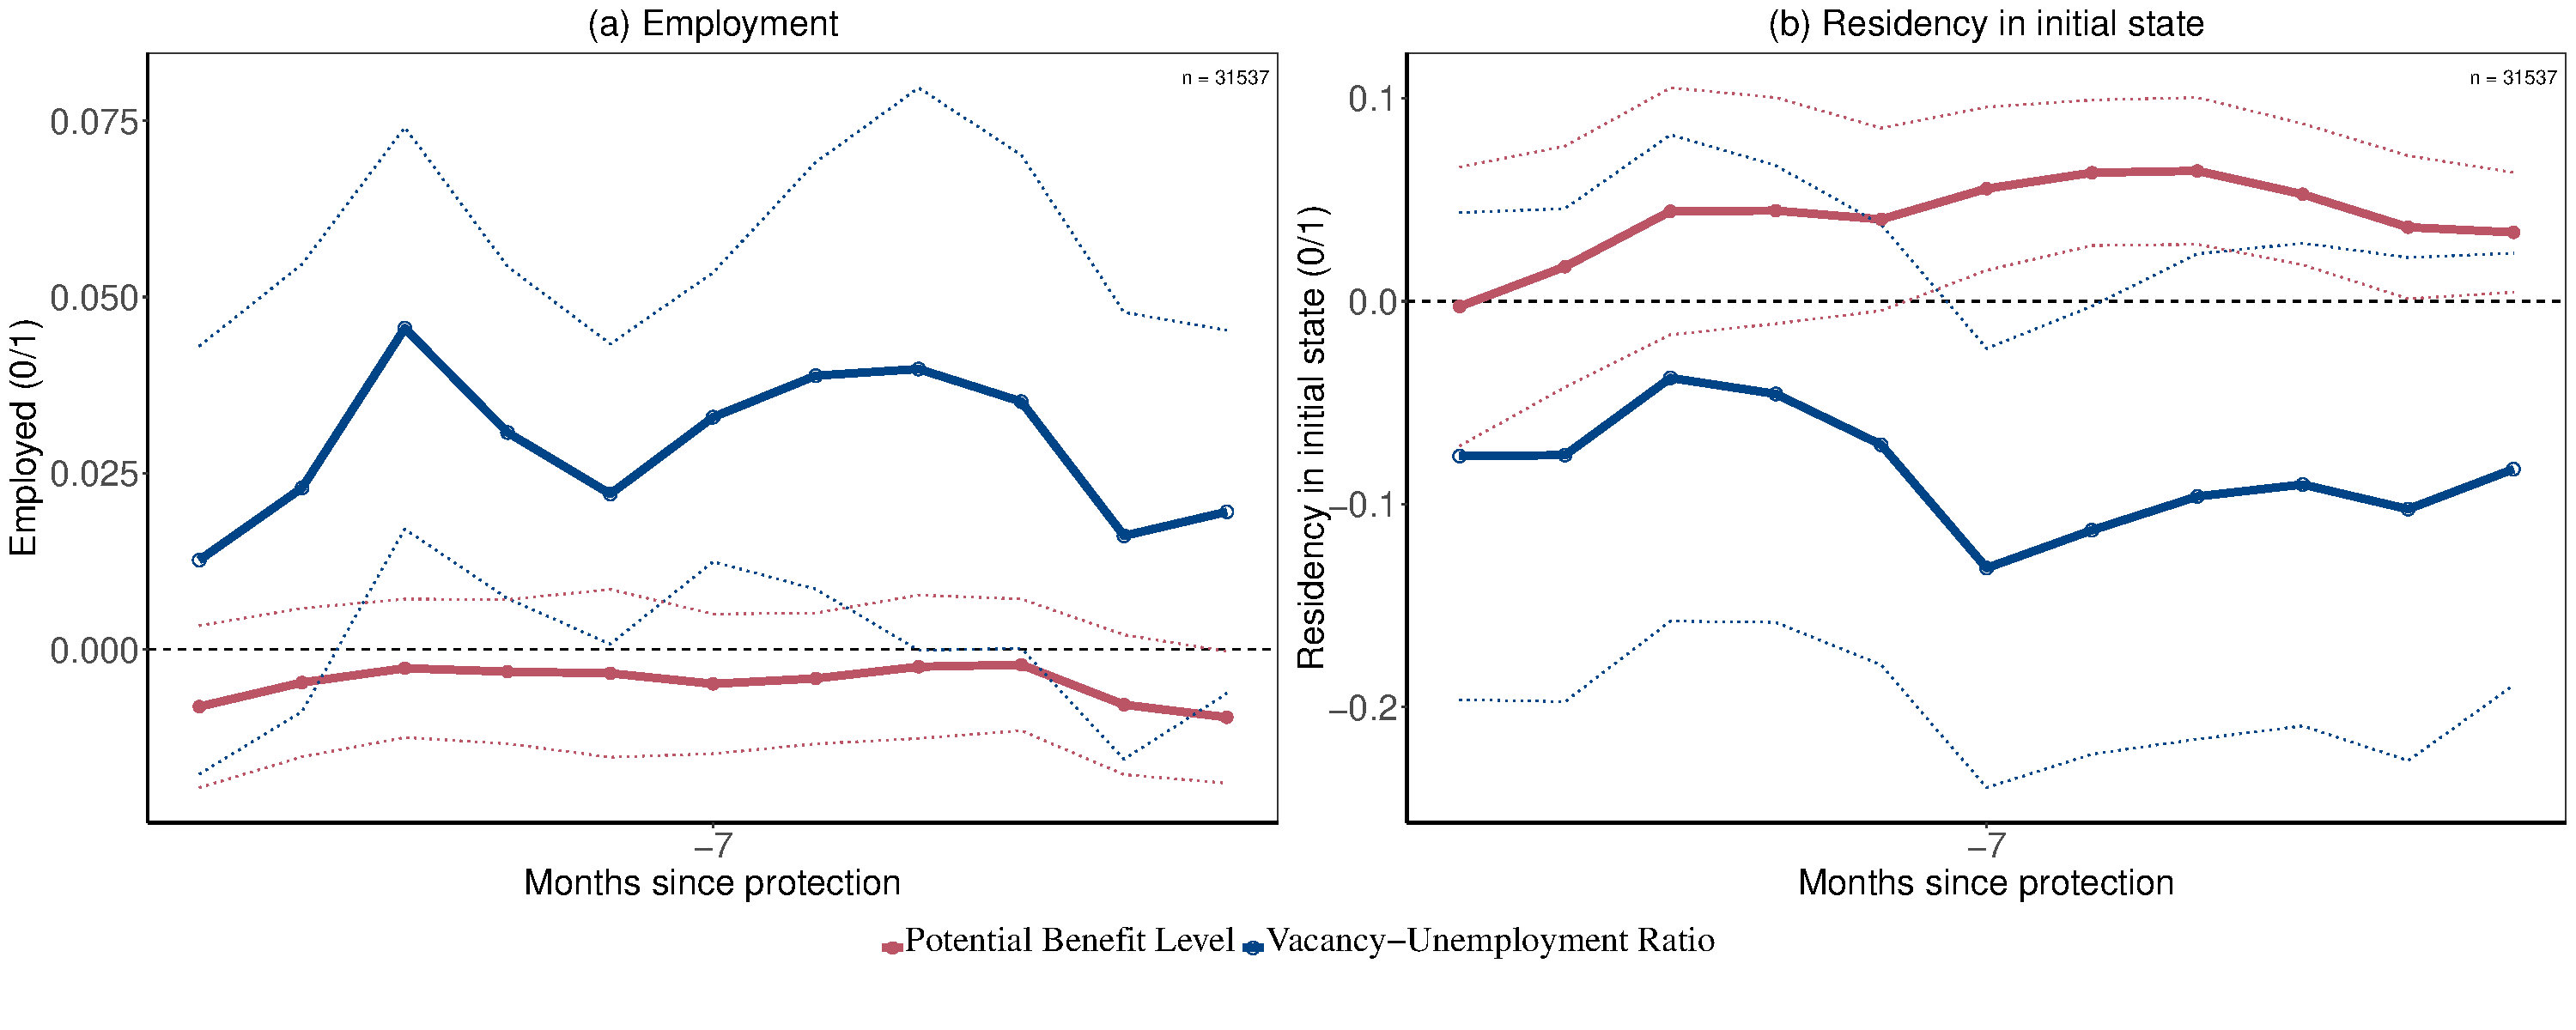
\includegraphics[scale=0.31]{figures/rob/fig_rob_labor_mobility_pre_trends_without_early_mover.pdf}
%     \end{center}
%     \fignote{Notes: The x-axis shows the months since protection was received. The y-axis displays the effect of a one-unit increase in either i) the vacancy-to-unemployment ratio or ii) the potential benefit level, measured in €1,000 (real 2015 values), on employment (left) and mobility (right). All regressions include a full set of arrival-group, year-month, and district-of-protection fixed effects. Additional control variables include age and age squared at immigration, gender, type of protection, family status at protection date, and country of origin. Standard errors are clustered at the district-year-of-protection level.}
% \end{figure}



% \begin{table}
%     \caption{Summary statistics excluding early movers}
%     \label{tab:summarystatistics_robustness}
%     \begin{threeparttable}
%         \begin{small}
%             \resizebox{\linewidth}{!}{%
%                 \begin{tabular}{lcccc}
%                     \expandableinput{figures/rob/descriptives_sample_without_early_movers.tex}
%                 \end{tabular}
%             }
%         \end{small}
%         \vspace{-1em}
%         \begin{tablenotes}
%             \parbox[t]{\textwidth}{%  % Set a strict width to the text width
%                 \fignote{Notes: The table reports means and standard deviations (in brackets) for continuous and binary variables. The number of observations and the percentage within groups are reported for categorical variables. Time-varying (outcome) variables are reported for the $12^th$ month after protection was received. The sample is restricted to refugees who received protection between January 2011 and August 2018, who were between 18 and 60 years old at the time of immigration and whose asylum process lasted longer than a day but less than three years, and where full data is available for 60 months after the date of protection. Family benefit eligibility is an indicator equal to one if children who are coinsured with this person or their partner are registered in Austria at the time of receiving protection. Duration asylum process is denoted in months and earnings are denoted in real 2015 euro.}
%             }
%         \end{tablenotes}
%     \end{threeparttable}
% \end{table}




%In Figure~\ref{fig:}, we further restrict the sample to asylum-seekers where we can confirm in the data that they were initially housed in one of the large reception centers. 
% initial placement
% standard errors

%\subsection{Event study analysis of individual reforms}
